\documentclass[a4paper,12pt]{article}

\usepackage[utf8]{inputenc}
\usepackage[left=0.5in,right=0.5in,top=1in,bottom=1in]{geometry}
\usepackage{amsmath,amssymb,amsfonts}
\usepackage{pgfplots,graphicx,calc,changepage}
\pgfplotsset{compat=newest}
\usepackage{enumitem}
\usepackage{fancyhdr}
\usepackage[colorlinks = true, linkcolor = blue]{hyperref}

% Syntax highlighting
\usepackage{listings}
\usepackage{xcolor}

\definecolor{codegreen}{rgb}{0.40,0.62,0.07}
\definecolor{codegray}{rgb}{0.5,0.5,0.5}
\definecolor{codeblue}{rgb}{0.09,0.57,0.73}
\definecolor{backcolour}{rgb}{1,1,1}

\lstdefinestyle{mystyle}{
    backgroundcolor=\color{backcolour},   
    commentstyle=\color{codegreen},
    keywordstyle=\color{magenta},
    numberstyle=\tiny\color{codegray},
    stringstyle=\color{codeblue},
    basicstyle=\ttfamily\small,
    breaklines=true,                     
    keepspaces=true,                 
    numbers=left,                    
    numbersep=5pt,                  
    showspaces=false,
    showstringspaces=false,
    showtabs=false,                  
    tabsize=4
}

\lstset{style=mystyle}

\newcommand{\nats}{\mathbb{N}}
\newcommand{\reals}{\mathbb{R}}
\newcommand{\rats}{\mathbb{Q}}
\newcommand{\ints}{\mathbb{Z}}
\newcommand{\pols}{\mathcal{P}}
\newcommand{\cants}{\Delta\!\!\!\!\Delta}
\newcommand{\eps}{\varepsilon}
\newcommand{\st}{\backepsilon}
\newcommand{\abs}[1]{\left| #1 \right|}
\newcommand{\dom}[1]{\mathrm{dom}\left(#1\right)}
\newcommand{\erf}{\mathrm{erf}}
\newcommand{\for}{\text{ for }}
\newcommand{\dd}{\mathrm{d}}
\newcommand{\spn}{\mathrm{sp}}
\newcommand{\nul}{\mathcal{N}}
\newcommand{\col}{\mathrm{col}}
\newcommand{\rank}{\mathrm{rank}}
\newcommand{\norm}[1]{\lVert #1 \rVert}
\newcommand{\inner}[1]{\left\langle #1 \right\rangle}
\newcommand{\pmat}[1]{\begin{pmatrix} #1 \end{pmatrix}}
\renewcommand{\and}{\text{ and }}

\newsavebox{\qed}
\newenvironment{proof}[2][$\square$]
{\setlength{\parskip}{0pt}\par\textit{Proof:} #2\setlength{\parskip}{0.25cm}
	\savebox{\qed}{#1}
	\begin{adjustwidth}{\widthof{Proof:}}{}
	}
	{
		\hfill\usebox{\qed}\end{adjustwidth}
}

\pagestyle{fancy}
\fancyhead{}
\lhead{Caleb Jacobs}
\chead{APPM 5600: Numerical Analysis I}
\rhead{Homework \#2}
\cfoot{}
\setlength{\headheight}{35pt}
\setlength{\parskip}{0.25cm}
\setlength{\parindent}{0pt}

\begin{document}
	\begin{enumerate}[label = \arabic*.]
		\item Which of the following iterations will converge to the indicated fixed point $ x_* $ (provided $ x_0 $ is sufficiently close to $ x_* $)? If it does converge, give the order of convergence; for linear convergence, give the rate of linear convergence.
		
		\begin{enumerate}[label = \roman*.]
			\item $ x_{n+1} = -16 + 6x_n + \frac{12}{x_n}, x_*= 2$
            
            Suppose
            \[
                x_{n+1} = g(x_n) = -16 + 6x_n + \frac{12}{x_n}.
            \]
            Then, Taylor expanding about $ x_* $ yields
            \[
                g(x_n) = g(x_*) + (6 - \frac{12}{\xi^2})(x_n - x_*) = x_* + (6 - \frac{12}{\xi^2})(x_n - x_*)
            \]
            for some $ \xi $ between $ x_n $ and $ x_* $. Using this expansion, we can get
            \begin{equation}
                \frac{\abs{x_{n + 1} - x_*}}{\abs{x_n - x_*}} =\abs{ 6 - \frac{12}{\xi^2}}. \label{equ:bad}
            \end{equation}
            Now, depending on our initial guess for $ x_n $, the RHS of (\ref{equ:bad}) can be greater than 1. For instance, suppose $ x_n = 3 $, then $ \xi \in [2, 3] $ which implies
            \[
               \frac{\abs{x_{n + 1} - x_*}}{\abs{x_n - x_*}} = \abs{ 6 - \frac{12}{\xi^2}} \geq 3.
            \]
            This shows that after an iteration near $ x_* $, the error actually grows larger. But, if we choose $ x_n = 1 $, then 
            \[
                \frac{\abs{x_{n + 1} - x_*}}{\abs{x_n - x_*}} = \abs{ 6 - \frac{12}{\xi^2}} \geq \frac{2}{3}
            \]
            Which shows that the error might decrease near $ x_* $. Putting these two points together shows that we are unsure if the iterate will converge or not provided $ x_0 $ is sufficiently close to $ x_* $.
			
			\item $ x_{n+1} = \frac{2}{3} x_n + \frac{1}{x_n^2}, x_* = 3^{1/3}$
			
			Suppose 
			\[
				g(x) = \frac{2}{3}x + \frac{1}{x^2}.
			\]
			Furthermore, suppose $ x_0 \in [1,2] $. Then $ x_* \in [1,2] $,  $ \min_{x \in [1,2]} g(x) = 3^{1/3} $, and $ \max_{x \in [1,2]}g(x) = \frac{5}{3} $. Therefore $ g([1,2]) \subset [1,2]$. So because $ g(x) $ is continuously differentiable on $ [1,2] $, Theorem 2.6 of Atkinson tells us that with $ x_0 \in [1,2] $ and $ x_{n+1} = g(x_n)$, that $ x_* $ is a unique solution to $ x = g(x) $ in $ [1,2] $ and that
			\[
				\lim_{n \to \infty} x_n = x_*.
			\]
			In other words, for any $ x_0 $ in the neighborhood $ [1,2] $ of $ x_* $, the fixed point iteration will converge.
			
			Now let's figure out the order of convergence. Taylor expanding $ g(x_n) $ about $ x_n = x_* $ yields
			\[
				x_{n+1} = g(x_n) = g(x_*) + \left(\frac{2}{3} - \frac{2}{x_*^3}\right)(x_n - x_*) + \frac{3}{\xi^4}(x_n - x_*)^2 = x_* + \frac{3}{\xi^4}(x_n - x_*)^2
			\]
			 for $ \xi $ between $ x_n $ and $ x_* $. Using the equality above, we can obtain
			\[
				\frac{\abs{x_{n+1} - x_*}}{\abs{x_n - x_*}^2} = \frac{3}{\xi^4}.
			\]
			Now because $ x_n \to x_* $ as $ n \to \infty $ and $ \xi $ is between $ x_n $ and $ x_* $, we must have $ \xi \to x_* $ as $ n \to \infty $. Thus
			\[
				\lim_{n \to \infty} \frac{\abs{x_{n+1} - x_*}}{\abs{x_n - x_*}^2} = \frac{3}{x_*^4}
			\]
			which shows that $ x_{n+1} = g(x_n) $ converges quadratically to $ x_* $ in the neighborhood $ [1,2] $.
			
			
			\item $ x_{n+1} = \frac{12}{1+x_n}, x_* = 3 $
			
			Just as in the previous part, let's first show that the iteration converges to $ x_* $ for $ x_0 $ sufficiently close to $ x_* $. First, let
			\[
				g(x) = \frac{12}{1+x} \text{ and } x_* = 3.
			\]
			Then $ x_{n+1} = g(x_n) $, $ x_* \in [2,4] $, $ \min_{x \in [2,4]}g(x) = \frac{12}{5} $, and $ \max_{x \in [2,4]} g(x) = 4$. Therefore, $ g([2,4]) \subset [2,4] $ and so by Theorem 2.6 on Atkinson, $ x_* $ is a unique solution to $ x = g(x) $ in $ [2,4] $ and any $ x_0 \in [2,4] $ with $ x_{n+1} = g(x_n)$ will have
			\[
				\lim_{n \to \infty}x_n = x_*.
			\]
			In other words, for any $ x_0 \in [2,4] $ (i.e. sufficiently close to $ x_* $), $ x_{n+1} = g(x_n) $ will converge to $ x_* $.
			
			Now let's determine the order and rate of convergence. Taylor expanding $ g(x_n) $ about $ x_n = x_* $ yields
			\[
				x_{n+1} = g(x_n) = g(x_*) - \frac{12}{(1+\xi)^2}(x_n - x_*)
			\]
			for some $ \xi $ between $ x_n $ and $ x_* $. Then, rearranging yields
			\[
				\frac{\abs{x_{n +1} - x_*}}{\abs{x_n - x_*}} = \abs{\frac{12}{(1 + \xi)^2}}.
			\]
			Finally, because $ \lim_{n\to\infty} x_n = x_*$, $  $$\lim_{n\to\infty} \xi = x_*$ and so
			\[
				\lim_{n \to \infty} \frac{\abs{x_{n +1} - x_*}}{\abs{x_n - x_*}} = \abs{\frac{12}{(1 + x_*)^2}} = \frac{3}{4}.
			\]
			This limit shows us that $ x_{n+1} = g(x_n) $ will converge linearly to $ x_* $ with a rate of $ \frac{3}{4} $ provided $ x_0 \in [2,4] $ (i.e. $ x_0 $ is sufficiently close to $ x_* $).
		\end{enumerate}
	
		\item In laying water mains, utilities must be concerned with the possibility of freezing. Although soil and weather conditions are complicated, reasonable approximations can be made on the basis of the assumption that soil is uniform in all directions.  In that case the temperature in degrees Celsius $ T(x,t) $ at a distance $ x $ (in meters) below the surface, $ t $ seconds after the beginning of a cold snap, approximately satisfies
		\[
			\frac{T(x,t) - T_s}{T_i - T_s} = \erf\left(\frac{x}{2\sqrt{\alpha t}}\right)34
		\]
		where $ T_s $ is the constant temperature during a cold period $ T_i $ is the initial soil temperature before the cold snap, $ \alpha $ is the thermal conductivity (in meters$ ^2 $) and 
		\[
			\erf(t) = \frac{2}{\sqrt{\pi}} \int_0^t e^{-s^2}\dd s
		\]
		Assume that $ T_i = 20 [\deg C]$, $ T_s = -15 [\deg C] $, $ \alpha = 0.138 \cdot 10^{-6} [$meters$ ^2 $ per second$ ] .$
        \begin{enumerate}[label = \roman*.]
            \item We want to determine how deep a water main should be buried so that it will only freeze after 60 days exposure at this constant surface temperature. Formulate the problem as a root finding problem $ f(x) = 0. $ What is $ f $ and what is $ f' $? Plot the function $ f $ on $ [0, \bar{x}] $, where $ \bar{x} $ is chosen so that $ f(\bar{x}) > 0 $. 
            
            First, let's identify what we are are trying to solve. We want to find $ x $ such that $ T(x, 60 [\text{days}]) = 0 $. To find, this, we to solve for $ T $ which yields
            \[
                T(x,t) = \erf\left(\frac{x}{2\sqrt{\alpha t}}\right) (T_i - T_s) + T_s.
            \]
            Setting this equation to zero reveals that our $ f $ is 
            \[
                f(x) = \erf\left(\frac{x}{2\sqrt{\alpha t}}\right) (T_i - T_s) + T_s
            \]
            with $ t = 60 [\text{days}] = 5184000 [\text{seconds}] $. Then,
            \[
                f'(x) = \frac{T_i - T_s}{\sqrt{\pi \alpha t}} e^{-\frac{1}{4 \alpha t} x^2}
            \]
            \begin{figure}[h!]
                \centering
                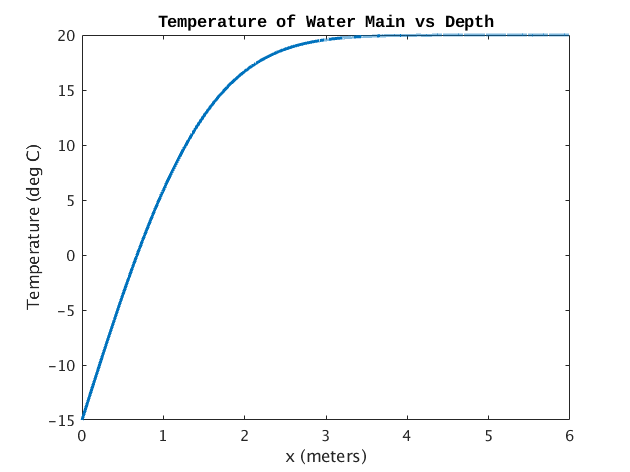
\includegraphics[width = 0.5\textwidth]{"images/WaterTemp.png"}
            \end{figure}
        
            \item Compute an approximate depth using the Bisection Method with starting values \\
            $ a_0 = 0 [\text{meters}] $ and $ b_0 = \bar{x} [\text{meters}] $.	
            
            Using $ a_0 = 0 $ and $ b_0 = \bar{x} = 6 $ with the bisection method converges to a root of\\
             $ x = .67696185448190249 $ after $ 46 $ iterations.
            
            \item Compute an approximate depth using Newton's Method with starting value $ x_0 = 0.01 [\text{meters}] $.
            
            Using $ x_0 = 0.01 $, Newton's method converges to a root of $ x = 0.6769618544819366 $ in $ 5 $ iterations. If instead we use $ x_0 = \bar{x} = 6 $, Newton fails after the first iteration due to a division by zero error. This faulty division is caused by our temperature function being flat away from the root and so when we used $ \bar{x} $, our derivative shot to zero which caused the next iteration to fly to another very flat section causing the code to throw an error. 
            
            Overall, I would still prefer Newton's method here because it converges much more rapidly than the bisection method (when it converges). Plus, in this case, when Newton wasn't going to work, it stopped only after a single iteration. Thus, it would still be faster to try another initial root guess for Newton than it would be to run the bisection method once.
            \begin{center}
                \textit{(Code used is at the end of the document)}
            \end{center}
            
        \end{enumerate}
        
		\item Consider applying Newton's method to a real cubic polynomial.
		\begin{enumerate}[label = \roman*.]
			\item In the case that the polynomial has three distinct real roots, $ x = \alpha, x = \beta, $ and $ x = \gamma $, show that the starting guess $ x_0 = \frac{1}{2} (\alpha + \beta) $ will yield the root $ \gamma $ in one step.
			
			Any cubic polynomial with roots $ x \in \{\alpha, \beta, \gamma \} $ can be written as
			\[
				p(x) = a (x - \alpha)(x - \beta)(x - \gamma)
			\]
			where $ a \in \reals $ is a constant. Using this general cubic yields a newton iteration of
			\[
				x_{n+1} = x_n - \frac{p(x_n)}{p'(x_n)}.
			\]
			Then, using $ x_0 = \frac{1}{2}(\alpha + \beta) $ yields an iteration of
			\begin{align*}
				x_1 = x_0 - \frac{p(x_0)}{p'(x_0)} &= \frac{1}{2}(\alpha + \beta)  - \frac{-\frac{1}{8} a (\alpha - \beta)^2 (\alpha + \beta - 2\gamma)}{-\frac{1}{4} a (\alpha - \beta)^2} \\
				&= \frac{1}{2}(\alpha + \beta)  - \frac{1}{2}(\alpha + \beta) + \frac{1}{2} (2\gamma) \\
				&= \gamma.
			\end{align*}
			Thus, $ x_1 = \gamma $ which shows Newton converges to $ x = \gamma $ in one iteration when $ x_0 = \frac{1}{2}(\alpha + \beta) $.
			
			\item Give a heuristic argument showing that if two roots coincide, there is precisely one starting guess $ x_0 $ other than $ x_0 = \beta $ for which Newton's method will fail, and that this one separates the basins of attraction for the distinct roots.
			
			Consider the cubic
			\[
				p(x) = a (x - \alpha)(x - \beta)^2
			\]
			with the constant $ a \in \reals$.  Any plot of $ p(x) $ will look similar to Figure \ref{fig:basin}. From the plot we can see that Newton fails whenever the derivative $ p'(x) = 0 $. One of these breaking points is the double root at $ \beta $; the other breaking point is at the $ x_b $ between $ \alpha $ and $ \beta $ for which $ p'(x_b) = 0 $. Now, Newton could potentially break at other points if after a certain iteration, we end up at $ x_b $ or $ \beta $. But, because we have a double root in this cubic, none of the tangent lines to $ p(x) $ cross the $ x $-axis at $ x_b $ or $ \beta $. This lack of other points is due to the function bouncing off the $ x $-axis at $ \beta $, because any tangent line constructed on $ p(x) $ will cross the $ x $-axis towards $ \alpha $ if $ x < x_b $ and will cross the $ x $-axis towards $ \beta $ if $ x > x_b $. Thus, any starting $ x_0 $ will move away $ x_b $. Even though iterations can move towards $ \beta $, they will never get to $ \beta $ and thus, won't break after a certain iteration.
			
			\begin{figure}[h!]
				\centering
				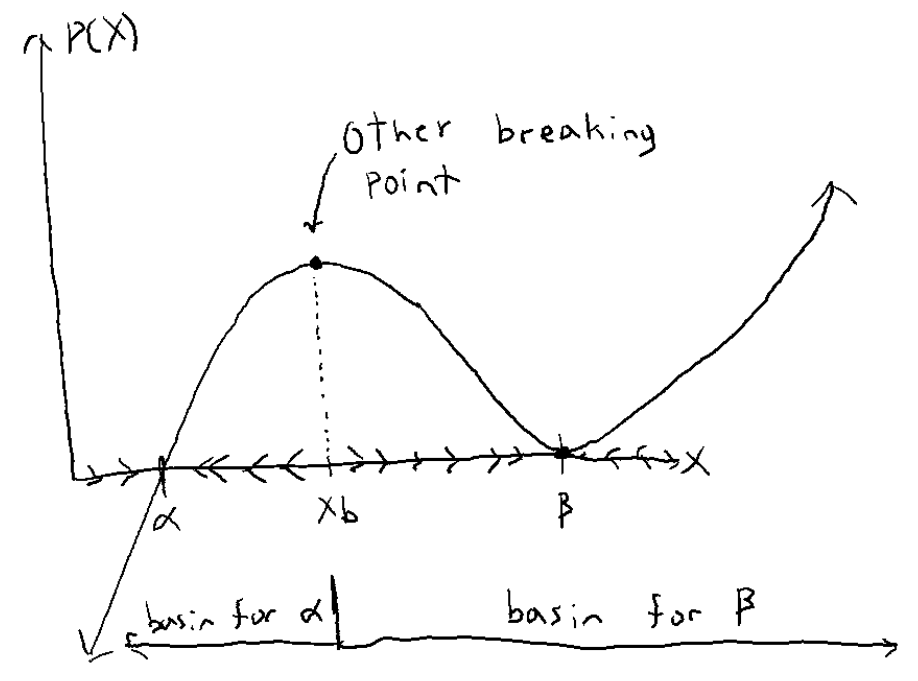
\includegraphics[width = 0.6\textwidth]{"images/Basin_of_attraction.png"}
				\caption{General plot of cubic polynomial with one double root}
				\label{fig:basin}
			\end{figure}
			
			From the discussion above and Figure \ref{fig:basin}, we can see that $ x_b $ forms the line between the basin of attraction for $ \alpha $ and $ \beta $ because the tangents cross the $ x $-axis closer to $ \alpha $ or $ \beta $ depending on if the initial $ x_0 $ is to the left or right of $ x_b $.
			
			\newpage
			\item Extend the argument in part ii. to the case when all three roots again are distinct.  Explain why there are now infinitely many starting guesses $ x_0 $ for which the iteration will fail.
			
			Consider the cubic polynomial:
			\[
				p(x) = a (x - \alpha)(x - \beta)(x - \gamma)
			\]
			where $ a \in \reals $ is a constant. All plots of $ p(x) $ will look similar to Figure \ref{fig:bad}. From Figure \ref{fig:bad}, we can see that we still have two obvious breaking points $ x_{b1} $ and $ x_{b2} $ between $ \alpha $ and $ \beta, $ and $ \beta $ and $ \gamma $. However, now both breaking points are not at roots. In fact, one breaking point will correspond to $ p(x) > 0 $, and one will correspond to $ p(x) < 0 $. Looking at where the tangent lines of $ p(x) $ cross the $ x $-axis show that there is a tangent line that crosses at $ x_{b1} $ and $ x_{b2} $. These tangents could send an initial point $ x_0 $ to one of the breaking points which would cause Newton to fail at the second iteration. Even worse, these new breaking points that map to the original breaking points have points that Newton will map to from somewhere else. We can keep repeating this process indefinitely to find an infinite sequence of points in a Newton iteration that will eventually work its way back to the first breaking points which will cause the method to fail. The light gray lines in Figure \ref{fig:bad} show a potential path that Newton can take to eventually break after some amount of iterations. 
			
			This sequence of breaking points only exists because the local max and min are on the opposite sides of the $ x $-axis and so the tangents will scan across the breaking points as $ x_n $ goes to the middle root from a local min or max.
			
			\begin{figure}[h!]
				\centering
				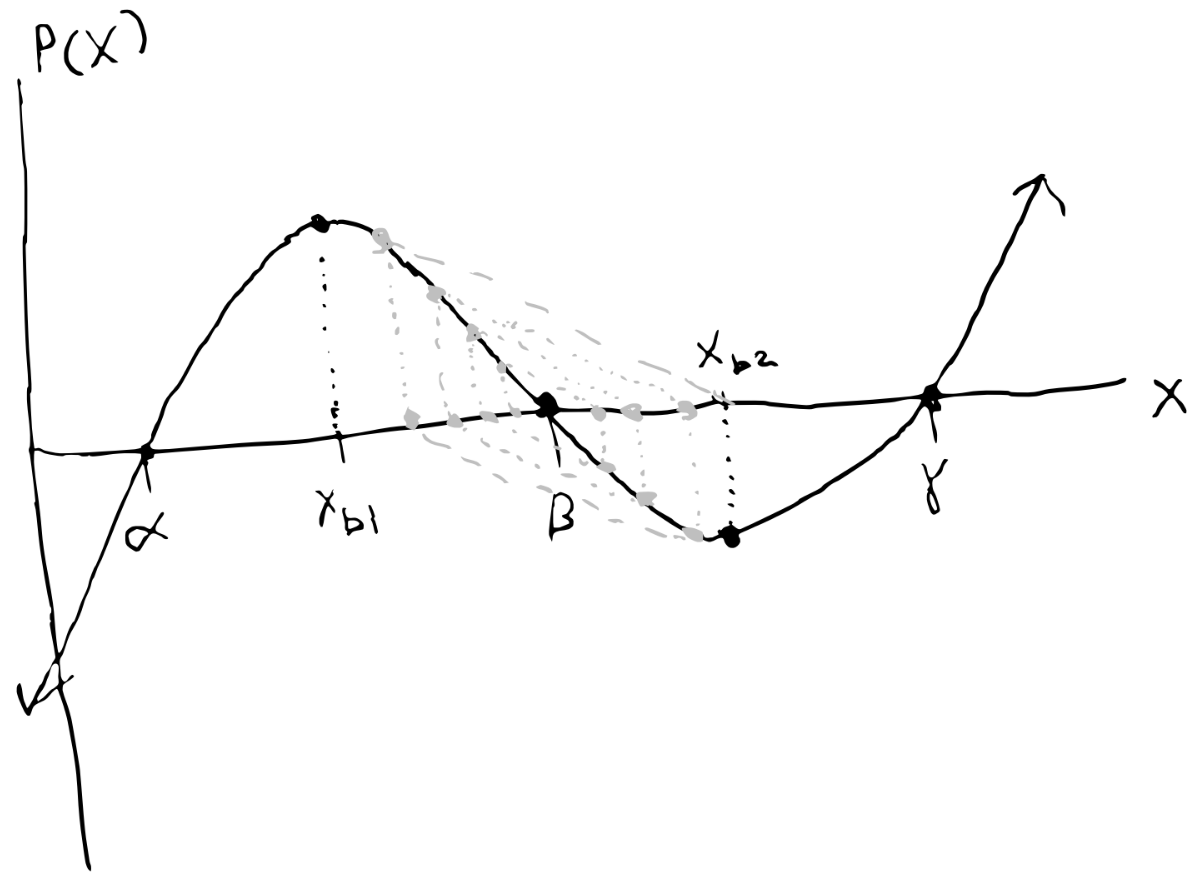
\includegraphics[width = 0.6\textwidth]{"images/Bad_points.png"}
				\caption{General plot of cubic polynomial with three distinct roots}
				\label{fig:bad}
			\end{figure}
		\end{enumerate}
	
		\newpage
		\item The sequence $ x_k $ produced by Newton's method is quadratically convergent to $ x_* $ with $ f(x_*) = 0 $, $ f'(x) \neq 0 $ and $ f''(x) $ continuous at $ x_* $.
		
		Let $ f(x) = (x-x_*)^p q(x) $ with $ p $ a positive integer with $ q $ twice continuously differentiable and $ q(x_*) \neq 0 $. Note: $ f'(x_*) = 0. $ In the following sub-problems, let $ x_k, f_k = f(x_k), e_k = \abs{x_* - x_k}, $ etc.
		
		\begin{enumerate}[label = \roman*.]
			\item Prove that Newton's method converges linearly for $ f(x). $
			
			Using $ f(x) = (x - x_*)^p q(x) $, we have the Newton iterate
			\[
				x_{n+1} = g(x_n) = x_n - \frac{f(x_n)}{f'(x_n)} = x_n - \frac{(x_n - x_*)q(x_n)}{p q(x_n) + (x_n - x_*)q'(x_n)}.
			\]
			Then,
			\begin{align*}
				\frac{\abs{x_{n+1} - x_*}}{\abs{x_n - x_*}} = \frac{\abs{g(x_n) - x_*}}{\abs{x_n - x_*}} &= \frac{\abs{x_n - x_* - \frac{(x_n - x_*)q(x_n)}{p q(x_n) + (x_n - x_*)q'(x_n)}}}{\abs{x_n - x_*}} \\
				&= \abs{1 - \frac{q(x_n)}{p q(x_n) + (x_n - x_*)q'(x_n)}}.
			\end{align*}
			Now, assuming $ \lim_{n -> \infty}x_n = x_* $, we can take the limit of both sides to get
			\[
				\lim_{x->x^*} \frac{\abs{x_{n+1} - x_*}}{\abs{x_n - x_*}} = \abs{1 - \frac{q(x_*)}{p q(x_*)}} = \abs{1 - \frac{1}{p}}
			\]
			which shows that Newton converges linearly.
			
			\item Consider the modified Newton iteration defined by 
			\[
				x_{k+1} = x_k - p \frac{f_k}{f_k'}.
			\]
			Prove that if $ x_k $ converges to $ x_* $, then the rate of convergence is quadratic.
            
            Firstly, let
            \[
                g(x_n) = x_n - p\frac{f(x_n)}{f'(x_n)} = x_n - p\frac{(x_n - x_*)q(x_n)}{p q(x_n) + (x_n - x_*)q'(x_n)}.
            \]
            Then,
            \begin{align*}
                \frac{\abs{x_{n+1} - x_*}}{\abs{x_n - x_*}^2} = \frac{\abs{g(x_n) - x_*}}{\abs{x_n - x_*}^2} &= \frac{\abs{x_n - x_* - p\frac{(x_n - x_*)q(x_n)}{p q(x_n) + (x_n - x_*)q'(x_n)}}}{\abs{x_n - x_*}^2} \\
                &= \frac{\abs{\frac{p(x_n - x_*)q(x_n) + (x_n - x_*)^2q'(x_n)}{p q(x_n) + (x_n - x_*)q'(x_n)} -\frac{p(x_n - x_*)q(x_n)}{p q(x_n) + (x_n - x_*)q'(x_n)}} }{\abs{x_n - x_*}^2} \\
                &= \frac{\abs{\frac{(x_n - x_*)^2q'(x_n)}{p q(x_n) + (x_n - x_*)q'(x_n)}}}{\abs{x_n - x_*}^2} \\
                &= \abs{\frac{q'(x_n)}{p q(x_n) + (x_n - x_*)q'(x_n)}}.
            \end{align*}
            Now, assuming $ x_n \to x_* $ as $ n \to \infty $, we have
            \[
                \lim_{n \to \infty}  \frac{\abs{x_{n+1} - x_*}}{\abs{x_n - x_*}^2} = \abs{\frac{q'(x_*)}{pq(x_*)}} = C
            \]
            where $ C > 0 $ is a constant. Therefore, the modified Newton method converges quadratically when $ x_n $ converges to $ x_* $.
				
			\item Write MATLAB codes for both Newton and modified Newton methods. Apply these to the function
			\[
				f(x) = (x-1)^5 e^x
			\]
			and compare the results. Use $ x_0 = 0 $ as a starting point.
            
            Running my \emph{Problem4.m} MATLAB code produces the figures:
            \begin{figure}[h!]
                \centering
                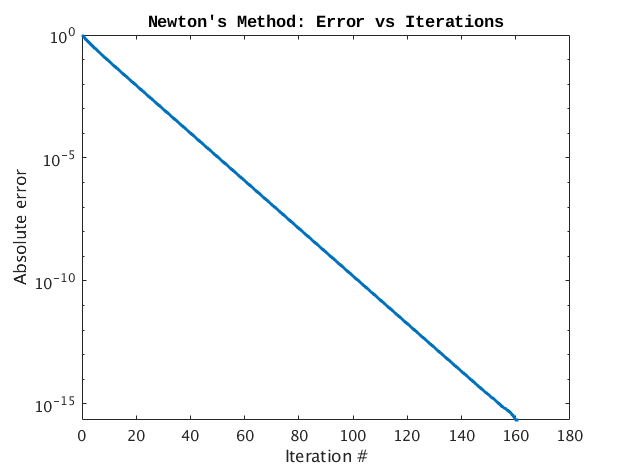
\includegraphics[width = 0.45\textwidth]{"images/Newton.png"}
                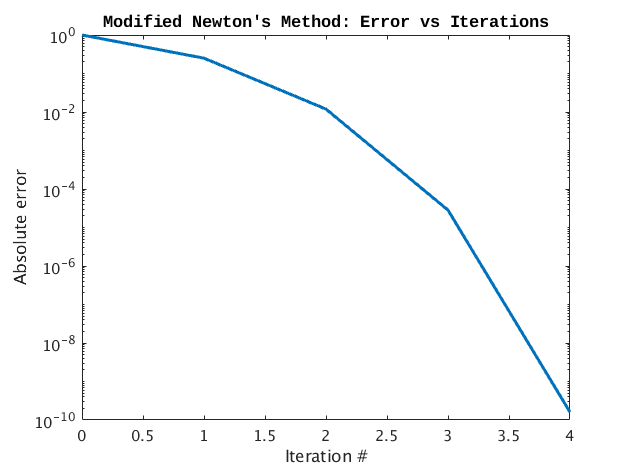
\includegraphics[width = 0.45\textwidth]{"images/Modified_Newton.png"}
            \end{figure}
            
            \newpage
            The accompanying data can be seen in the tables below:
            
            Convergence table for Newton's Method
            \begin{verbatim}
-------x value---------------Absolute Error----
0                    	    1.000000000000000e+00
2.500000000000000e-01     7.500000000000000e-01
4.264705882352942e-01     5.735294117647058e-01
5.560386945475865e-01     4.439613054524135e-01
6.534832807807371e-01     3.465167192192629e-01
7.279472249514199e-01     2.720527750485801e-01
7.854886403066591e-01     2.145113596933409e-01
8.303140230035438e-01     1.696859769964562e-01
8.654434113183316e-01     1.345565886816684e-01
8.930989767635392e-01     1.069010232364608e-01
9.149462812517817e-01     8.505371874821832e-02
9.322513979063947e-01     6.774860209360534e-02
9.459872350785150e-01     5.401276492148499e-02
9.569077575858133e-01     4.309224241418674e-02
9.656011294461713e-01     3.439887055382873e-02
9.725285627331186e-01     2.747143726688139e-02
9.780532041545410e-01     2.194679584545900e-02
9.824619147378555e-01     1.753808526214451e-02
9.859818784751131e-01     1.401812152488691e-02
9.887933851886461e-01     1.120661481135388e-02
9.910397429641806e-01     8.960257035819374e-03
9.928350115850026e-01     7.164988414997353e-03
9.942700656972199e-01     5.729934302780126e-03
9.954173673503955e-01     4.582632649604457e-03
9.963347346718042e-01     3.665265328195777e-03
9.970683254984478e-01     2.931674501552184e-03
9.976550043890671e-01     2.344995610932932e-03
9.981242235746398e-01     1.875776425360187e-03
9.984995196540195e-01     1.500480345980493e-03
9.987997058079005e-01     1.200294192099549e-03
9.990398222884037e-01     9.601777115962884e-04
9.992318947154557e-01     7.681052845442959e-04
9.993855393754196e-01     6.144606245803708e-04
9.995084466046663e-01     4.915533953336881e-04
9.996067669496730e-01     3.932330503270132e-04
9.996854197455142e-01     3.145802544858300e-04
9.997483397550898e-01     2.516602449101901e-04
9.997986743375146e-01     2.013256624854298e-04
9.998389410913578e-01     1.610589086421532e-04
9.998711539107186e-01     1.288460892814314e-04
9.998969237926446e-01     1.030762073553904e-04
9.999175394591127e-01     8.246054088734134e-05
9.999340318392842e-01     6.596816071580136e-05
9.999472256455015e-01     5.277435449846379e-05
9.999577806278077e-01     4.221937219228700e-05
9.999662245735458e-01     3.377542645421894e-05
9.999729797044681e-01     2.702029553192098e-05
9.999783837927785e-01     2.161620722151980e-05
9.999827070529133e-01     1.729294708674445e-05
9.999861656542924e-01     1.383434570756403e-05
9.999889325310896e-01     1.106746891044175e-05
9.999911460297712e-01     8.853970228761554e-06
9.999929168269527e-01     7.083173047317537e-06
9.999943334635690e-01     5.666536430970481e-06
9.999954667721396e-01     4.533227860425981e-06
9.999963734185336e-01     3.626581466353862e-06
9.999970987353530e-01     2.901264646970603e-06
9.999976789886191e-01     2.321011380868043e-06
9.999981431911108e-01     1.856808889200146e-06
9.999985145530266e-01     1.485446973426008e-06
9.999988116425095e-01     1.188357490522485e-06
9.999990493140640e-01     9.506859359742492e-07
9.999992394512873e-01     7.605487126749466e-07
9.999993915610530e-01     6.084389470029095e-07
9.999995132488572e-01     4.867511428363613e-07
9.999996105990953e-01     3.894009047433755e-07
9.999996884792822e-01     3.115207177772916e-07
9.999997507834296e-01     2.492165703804616e-07
9.999998006267462e-01     1.993732537952653e-07
9.999998405013986e-01     1.594986014374911e-07
9.999998724011199e-01     1.275988801285877e-07
9.999998979208965e-01     1.020791035033497e-07
9.999999183367176e-01     8.166328235859055e-08
9.999999346693744e-01     6.533062557600999e-08
9.999999477354997e-01     5.226450028317231e-08
9.999999581883999e-01     4.181160007110662e-08
9.999999665507200e-01     3.344928001247638e-08
9.999999732405760e-01     2.675942400998110e-08
9.999999785924608e-01     2.140753918578042e-08
9.999999828739686e-01     1.712603137082880e-08
9.999999862991750e-01     1.370082503004966e-08
9.999999890393400e-01     1.096066004624419e-08
9.999999912314720e-01     8.768528014790888e-09
9.999999929851776e-01     7.014822389628250e-09
9.999999943881421e-01     5.611857867293679e-09
9.999999955105137e-01     4.489486338243864e-09
9.999999964084110e-01     3.591589026186170e-09
9.999999971267288e-01     2.873271176540015e-09
9.999999977013830e-01     2.298616963436473e-09
9.999999981611064e-01     1.838893592953639e-09
9.999999985288851e-01     1.471114896567371e-09
9.999999988231081e-01     1.176891917253897e-09
9.999999990584865e-01     9.415135338031178e-10
9.999999992467892e-01     7.532108270424942e-10
9.999999993974313e-01     6.025686616339954e-10
9.999999995179450e-01     4.820549515116568e-10
9.999999996143560e-01     3.856439612093254e-10
9.999999996914848e-01     3.085152133763813e-10
9.999999997531879e-01     2.468121262921841e-10
9.999999998025503e-01     1.974497232382078e-10
9.999999998420402e-01     1.579597563861057e-10
9.999999998736322e-01     1.263678051088846e-10
9.999999998989058e-01     1.010942440871077e-10
9.999999999191246e-01     8.087541747414662e-11
9.999999999352996e-01     6.470035618377779e-11
9.999999999482397e-01     5.176026274256174e-11
9.999999999585918e-01     4.140821019404939e-11
9.999999999668734e-01     3.312661256416050e-11
9.999999999734988e-01     2.650124564240741e-11
9.999999999787990e-01     2.120104092284691e-11
9.999999999830391e-01     1.696087714719852e-11
9.999999999864313e-01     1.356870171775881e-11
9.999999999891450e-01     1.085498357866754e-11
9.999999999913161e-01     8.683942454013049e-12
9.999999999930529e-01     6.947109554289455e-12
9.999999999944423e-01     5.557665438971071e-12
9.999999999955539e-01     4.446110146716364e-12
9.999999999964431e-01     3.556932526294077e-12
9.999999999971545e-01     2.845501612114276e-12
9.999999999977236e-01     2.276401289691421e-12
9.999999999981789e-01     1.821098827292644e-12
9.999999999985432e-01     1.456834652913130e-12
9.999999999988345e-01     1.165512131251489e-12
9.999999999990676e-01     9.323652960802065e-13
9.999999999992542e-01     7.458478279431802e-13
9.999999999994034e-01     5.966338534335591e-13
9.999999999995227e-01     4.772848782863548e-13
9.999999999996182e-01     3.818056981685913e-13
9.999999999996946e-01     3.054223540743806e-13
9.999999999997556e-01     2.443600877199970e-13
9.999999999998045e-01     1.955102746364901e-13
9.999999999998436e-01     1.564304241696846e-13
9.999999999998749e-01     1.251221348752551e-13
9.999999999998999e-01     1.001421168211891e-13
9.999999999999198e-01     8.015810237793630e-14
9.999999999999358e-01     6.417089082333405e-14
9.999999999999487e-01     5.129230373768223e-14
9.999999999999589e-01     4.107825191113079e-14
9.999999999999671e-01     3.286260152890463e-14
9.999999999999737e-01     2.631228568361621e-14
9.999999999999789e-01     2.109423746787797e-14
9.999999999999831e-01     1.687538997430238e-14
9.999999999999865e-01     1.354472090042691e-14
9.999999999999891e-01     1.088018564132653e-14
9.999999999999913e-01     8.659739592076221e-15
9.999999999999931e-01     6.883382752675971e-15
9.999999999999944e-01     5.551115123125783e-15
9.999999999999956e-01     4.440892098500626e-15
9.999999999999964e-01     3.552713678800501e-15
9.999999999999971e-01     2.886579864025407e-15
9.999999999999977e-01     2.331468351712829e-15
9.999999999999981e-01     1.887379141862766e-15
9.999999999999984e-01     1.554312234475219e-15
9.999999999999988e-01     1.221245327087672e-15
9.999999999999990e-01     9.992007221626409e-16
9.999999999999992e-01     7.771561172376096e-16
9.999999999999993e-01     6.661338147750939e-16
9.999999999999994e-01     5.551115123125783e-16
9.999999999999996e-01     4.440892098500626e-16
9.999999999999997e-01     3.330669073875470e-16
9.999999999999998e-01     2.220446049250313e-16
9.999999999999998e-01     2.220446049250313e-16
             \end{verbatim}
            
            Convergence table for Modified Newton's Method:
            \begin{verbatim}
-------x value---------------Absolute Error----
0                    	    1.000000000000000e+00
1.250000000000000e+00     2.500000000000000e-01
1.011904761904762e+00     1.190476190476186e-02
1.000028277344192e+00     2.827734419175165e-05
1.000000000159921e+00     1.599207433145011e-10
1.000000000000000e+00                         0
            \end{verbatim}
        
        From the error plots and tables, clearly the Modified Newton's method converges much faster (in only 5 iterations vs 161 iterations from Newton's method). But, to really understand what's happening, we can first turn to the tables. The Newton's method table shows an error that is decreasing at a nearly linear rate with the method gaining another power of ten of accuracy every ten or so iterations. Similarly, the plot of Newton's method shows a straight line when we logarithmically scale the $ y $-axis. Both of these combined tell us that Newton's method is converging to the multiple root linearly. 
        
        On the other hand, the table of the Modified Newton's method shows the number of digits that we have correct doubles after each iteration (just like quadratic convergence in the theory describes). Furthermore, the error plot of the Modified Newton's method shows a decreasing, concave down curve as the number of iterations increases with a logarithmically scaled $ y $-axis. This type of downward curve is characteristic of higher order methods which only support the theory more that the Modified Newton's method has quadratic convergence.
	\end{enumerate}
\end{enumerate}

\newpage
\begin{center}
    \textbf{Problem 2 Code}
\end{center}
\rule{\textwidth}{0.4pt}
\lstinputlisting[language = matlab]{"code/Problem2.m"}
\rule{\textwidth}{0.4pt}

\newpage
\begin{center}
    \textbf{Problem 4 Code}
\end{center}
\rule{\textwidth}{0.4pt}
\lstinputlisting[language = matlab]{"code/Problem4.m"}
\rule{\textwidth}{0.4pt}

\newpage
\begin{center}
    \textbf{Bisection Code}
\end{center}
\rule{\textwidth}{0.4pt}
\lstinputlisting[language = matlab]{"code/bisection.m"}
\rule{\textwidth}{0.4pt}

\newpage
\begin{center}
    \textbf{Newton's Method Code}
\end{center}
\rule{\textwidth}{0.4pt}
\lstinputlisting[language = matlab]{"code/newton.m"}
\rule{\textwidth}{0.4pt}
\end{document}